\documentclass{article}

% Language setting
% Replace `english' with e.g. `spanish' to change the document language
\usepackage[francais]{babel}

% Set page size and margins
% Replace `letterpaper' with`a4paper' for UK/EU standard size
\usepackage[a4paper,top=2cm,bottom=2cm,left=3cm,right=3cm,marginparwidth=1.75cm]{geometry}

% Useful packages
\usepackage{amsmath}
\usepackage{amsfonts}
\usepackage{fancyhdr}
\usepackage{graphicx}
\usepackage[T1]{fontenc}
\usepackage{alertmessage}
\usepackage{float}
\usepackage{subfig}
\usepackage[colorlinks=false, allcolors=blue]{hyperref}

\title{
    \underline{MAT 41 02} \\
    Apprentissage Non Supervisé - Application sur la base de données MNIST
}
\author{Charles Farhat et TERPEREAU Léopold}

\pagestyle{fancy}
\renewcommand{\headrulewidth}{0.2pt}
\renewcommand{\footrulewidth}{0.2pt}
\fancyhead[L]{}
\fancyhead[R]{\textit{Apprentissage Non Supervisé - MNIST}}
\fancyfoot[C]{\thepage}
\fancyfoot[R]{TP MNIST - Charles Farhat}



\begin{document}
\maketitle

\begin{figure}[h]
    \centering
    
\includegraphics[scale=0.22]{Images/1024-1318.png}
\end{figure}


\newpage
\vspace*{\stretch{1}}
\begin{center}

    \tableofcontents
    %Pour qu'une section ne soit pas prise en compte dans la table des matières il suffit d'écrire 
    %\section*{Titre de la section}
\end{center}
\vspace*{\stretch{1}}


\newpage


\section{Introduction}
Ce rapport fait suite à la réalisation du cours \textit{Introduction aux méthodes de classifications non supervisées} du modules \textbf{MAT 4102} de Télécom SudParis. \newline
Dans ce rapport il sera question de la très connue base de données MNIST, ce TP porte donc sur la plus classique introduction à de l'apprentissage machine : la classification de chiffres écrits à la main.  

La spécificité tiens à l'approche qui sera utilisée pour la classification : nous chercherons à la réaliser à partir de méthodes usuellement appliquées à des problèmes non supervisés. 
Par ailleurs, il est imposé d'utiliser les algorithmes \textit{Kmeans} et \textit{Kmedoids}, le contenu portera donc sur la comparaison des résultats de ces deux algorithmes dans différents contextes.

\vspace{2mm}
Il est également demandé à ce que ce rapport soit succint. Nous considérons donc que certains des principes et fonctionnements de bases des deux algorithmes sont connus et nous nous concentrerons uniquement sur ce qui a été apporté.


\newpage

\section{Découverte des algorithmes et première approche}
\vspace{4mm}

Le but de ce TP n'est pas de développer à proprement parler les algorithmes Kmeans et Kmedoids mais de les analyser. Toute références à ces deux fontions sera issue de la librairie \textit{Scikit Learn},  \url{https://scikit-learn.org/stable/}. La base de données utilisée est elle aussi issue de la librarie \textit{sklearn}. Elle est composée de $70000$ matrices représentants des chiffres de 0 à 9 sur des images en niveaux de gris de 784 pixels (28*28, 1 dimension, pixels valants 0 à 255). Dans ce TP nous ne considérons que les 10 000 premières images.

\begin{center}
  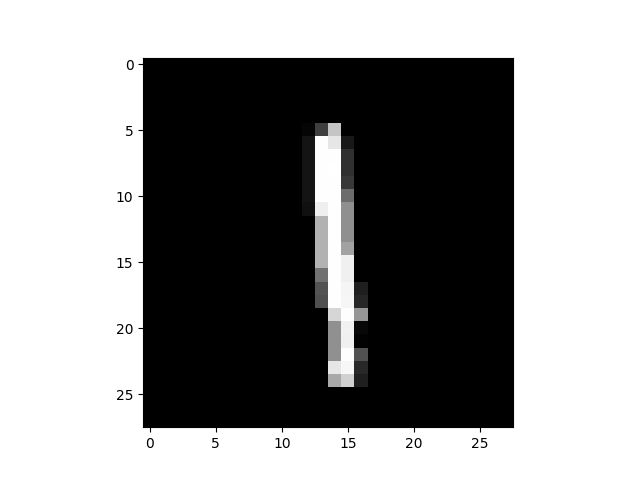
\includegraphics[width=0.3\textwidth]{"./Images/1.png"}
  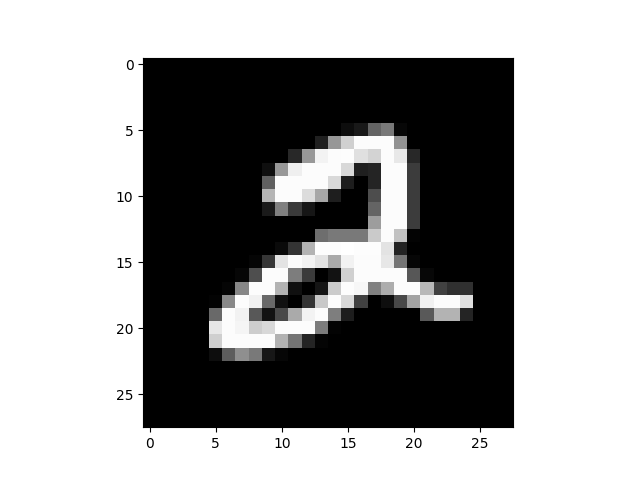
\includegraphics[width=0.3\textwidth]{"./Images/2.png"}
  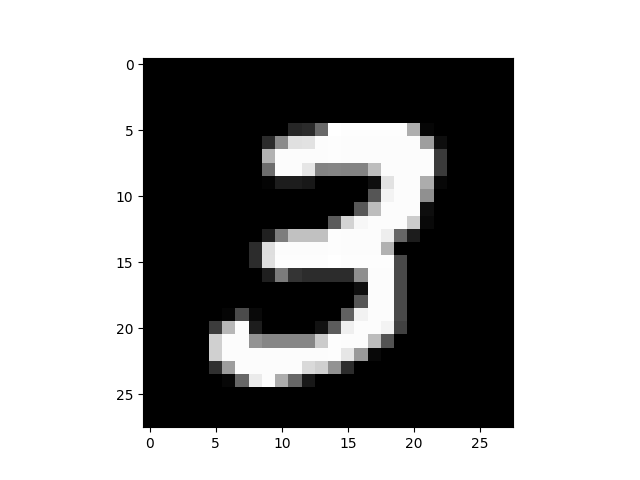
\includegraphics[width=0.3\textwidth]{"./Images/3.png"}
\end{center}

%Quelques images issues de la base de données.


\textit{Dans toute notre étude nous utiliserons les paramètres par défault proposés par sklearn,  notamment $n\_init$ et $max\_iter$ qui correspondent respectivement au nombre d'initialisationx à considérer (Kmeans étant fortement non convexe, son état initial a un grande influence sur le résultat final) et au nombre d'itérations maximales (pour le calcul de position des barycentres) s'il ne semble pas y avoir convergence "rapide" de l'inertie. \newline La détermination des hyperparamètres étant surtout un enjeux pour l'augmentation des performances, et n'étant pas la problématique ici...}

\subsection{Observation et Premiers résultats}

\subsubsection{Observation}

La première chose qu'il tient à faire, surtout dans le cas d'apprentissage non supervisé, est de chercher à représenter les données, de rendre visuel ce que nous cherchons à trier. classifier. Nous sommes ici chanceux : même si l'on supposait ne pas connaître la classe de chaque matrice à l'avance, visualiser des images de cette simplicité (niveau de gris) et en déduire des tendances est une tâche relativement aisée. \\
Quelques remarques peuvent rapidement être formulées après une première observation du dataset : 

\begin{enumerate}
    \item Les images ne sont pas centrées.
    \item L'immense majorité des images contient une bordure de noir lorsque l'on s'approche des bords. Cette bordure varie de 3 à 7/8 pixels.
    \item Certaines images contiennent principalement des niveaux de gris aux endroits représentants leur chiffre.
\end{enumerate}

Aux yeux de Kmeans et Kmedoids nos images sont simplements des vecteurs de 784 coordonnées. Le but des deux programmes est de déterminer des frontières permettants de séparer ces vecteurs en $n \in \mathbb{N}^*$ groupes, le tout en minimisant un critère appelé \textit{Inertie}. 
\\
Comme nous venons de le mentionner, presque toutes les images admettent des pixels noirs lorsque nous nous rapprochons des positions extrêmes. Une telle propriété n'est pas discrimante et donc d'aucune utilité pour les deux algorithmes, c'est pourquoi nous proposons donc de réduire les image à des matrices 22*22 en supprimant les 3 premières et dernières lignes, ainsi que les 3 premières et dernières colonnes. \\

Une fois ce premier traitement réalisé, nous avons certes réduit la quantité d'informations disponibles (vecteurs de 784 coordonnées à vecteurs de 484 coordonnées) mais nous avons surtout augmenté la qualité de nos données. Ce type de transformation est souvent recherché en apprentissage machine car il permet de réduire le temps de calcul tout en augmentant les performances. 

\newpage

\subsubsection{Premiers résultats}

A l'aide du notebook fourni et des implémentations de Kmeans et Kmedoids de sklearn nous pouvons passer à l'analyse des premiers résultats obtenu.

\alertinfo{Dans le cas de MNIST les données sont déjà comparables à l'état brut, il ne semble donc pas particulièrement important de les standardiser. D'autant plus que le but est davantage d'introduire à de nouvelles notions que d'arriver à des performances intéressantes (d'autant plus qu'il s'agit de MNIST...). Nous diviserons tout de même tous les pixels par 255 pour les normaliser, afin d'avancer avec des grandeurs plus petites.}

Après une première classification par l'algorithme de Kmeans, nous pouvons observer les barycentre de nos différents clusters :

\begin{figure}[H]
	\centering
	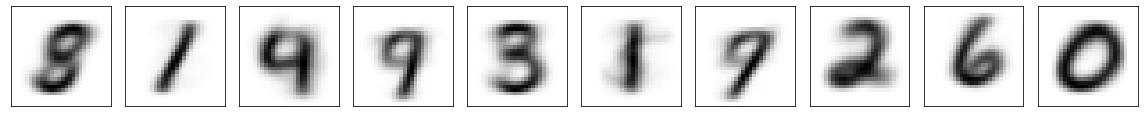
\includegraphics[width=0.8\textwidth]{"./Images/centre_clusters.png"}
	\caption{Représentation des centres des cluster du Kmeans (avec K=10)}
	\label{fig:centerClusters}
\end{figure}

On remarque donc qu’en choisissant de manière logique 10 clusters, on ne retrouve pas les centres des classes qu’on s’attendait à avoir (c’est-à-dire une représentation des 10 chiffres), bien qu’on retrouve 7 classes de chiffres différents. Il nous vient alors d'avancer que face à la ressemblance de certains chiffres entre 0 et 9 (8 et 3 ou 9 et 4) l'algorithme du Kmeans n'est pas assez robuste. Il nous faudra donc augmenter le nombre de clusters pour essayer de distinguer plus subtilement les différences entre classes. Puis regrouper nos résultats. \\

\paragraph{Question de coût} Nous allons maintenant nous intéresser à la fonction de coût du Kmeans. Dans notre cas sa fonction de coût est définie comme :

\begin{equation}
	\begin{cases}
		\mathbf{J} =\sum _{i=1}^{K}\sum _{x\in ClusterC_{i}}\Vert ( x-m_{i})\Vert ^{2}\\
		\\\\
		m_{i} =\frac{1}{n}\sum _{x\in ClusterC_{i}} x\ \ \ :\ i^{eme} \ centre\\
		\\\\
		n_{i} \ :\ Nombre\ des\ données\ assignées\ au\ clusterC_{i}
	\end{cases}
\end{equation}
\begin{center}	
\end{center}

On obtient alors :
\begin{figure}[H]
	\centering
	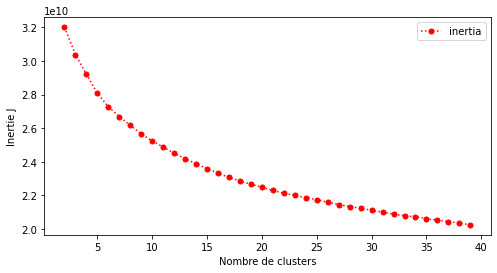
\includegraphics[width=0.8\textwidth]{"./Images/inertia.png"}
	\caption{Inertie du modèle en fonction du nombre de clusters (K)}
	\label{fig:inertia}
\end{figure}

\alertinfo{L'inertie diminue avec le nombre de cluster, ce qui est cohérent. Dans la littérature on trouve que les applications sérieuses de Kmeans utilisent 200 clusters pour la classifications de MNIST, les résultats que nous obtenons tendent bien dans ce sens.}

Pour nous aider dans notre prise de décision (pour le meilleur nombre de cluster), nous allons nous aider de la silouhette. La silhouette est une mesure de la similitude d’un objet avec son propre cluster (cohésion) par rapport à d’autres clusters (séparation). Elle va de -1 à 1, où une valeur proche de 1 indique une bonne correspondance entre l’objet et son propre cluster, tandis qu’une valeur proche de -1 indique une meilleure correspondance de l’objet avec un autre cluster. Si la valeur moyenne de la silhouette est élevée, cela indique que les amas sont bien séparés et que les objets sont bien regroupés.
Lors de l’application de l’algorithme k-means, la silhouette peut être utilisée pour déterminer le nombre optimal de clusters. L’algorithme est initialisé avec un certain nombre de clusters k, et la valeur de silhouette moyenne pour chaque objet est calculée. Ensuite, la valeur moyenne globale de la silhouette pour tous les objets du jeu de données est calculée. Le processus est répété pour différentes valeurs de k, et la valeur de silhouette moyenne est notée pour chaque k.

\begin{figure}[H]
	\centering
	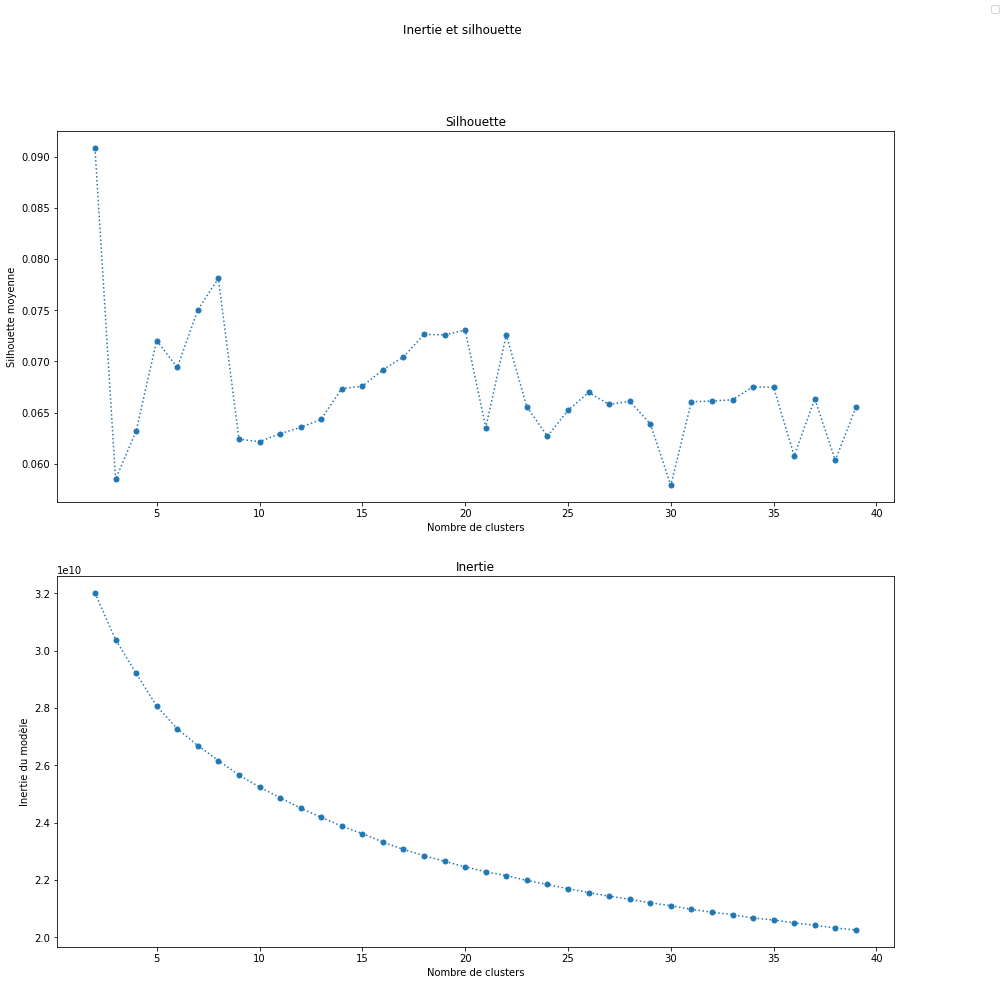
\includegraphics[width=0.85\textwidth]{"./Images/silouhette.png"}
	\caption{Siouhette moyenne du modèle en fonction du nombre de clusters (K)}
	\label{fig:sil}
\end{figure}

Le nombre optimal de clusters est celui qui maximise la valeur moyenne globale de la silhouette. Plus précisément, le nombre de clusters pour lesquelles la valeur moyenne globale de la silhouette est maximale est celui qui fournit le meilleur partitionnement de l’ensemble de données. Dans notre cas, ce nombre semble être 7, si on ne prend pas en compte la valeur de départ (2 n'offrant pas un bon partitionnement des données !).

\newpage

\subsubsection{Nouvelles métriques}

L'inertie et la silhouette présentées dans la partie précédente sont des indicateurs certe intéressants pour ce type de situation mais leur analyse seule (valeur et vitesse de convergence) manque d'information, c'est pourquoi il existe d'autres indicateurs permettant de décider si une classification est non seulement 'bonne' mais également 'correctement paramétrée'.  \\

Nous avons choisi d'utiliser les deux mesures suivantes : $\textit{le critère de David Bourdin}$ [1] et celui de $\textit{le critère de Calinski Harabasz}$ [2].

\paragraph{Calinski Harabasz} L'indice de Calinski-Harabasz permet une mesure du rapport de la variance entre-clusters sur la variance intra-cluster, et est calculé comme suit :

$$CH(k) = \frac{B(k) / (k - 1)}{W(k) / (n - k)}$$

où $k$ est le nombre de clusters, $n$ est le nombre total de points de données, $B(k)$ est la variance entre-clusters et $W(k)$ est la variance intra-cluster. \\

L'idée derrière l'indice de Calinski-Harabasz est qu'une bonne solution de clustering aura une variance entre-clusters élevée et une variance intra-cluster faible, ce qui signifie que les clusters sont bien séparés les uns des autres et que les objets dans chaque cluster sont similaires les uns aux autres. L'indice prend en compte à la fois la compacité et la séparation des clusters, et fournit donc une mesure équilibrée de la qualité du clustering. \\

Pour déterminer le nombre optimal de clusters, on peut calculer l'indice de Calinski-Harabasz pour différentes valeurs de $k$ et choisir la valeur de $k$ qui maximise l'indice.
\begin{figure}[H]
	\centering
	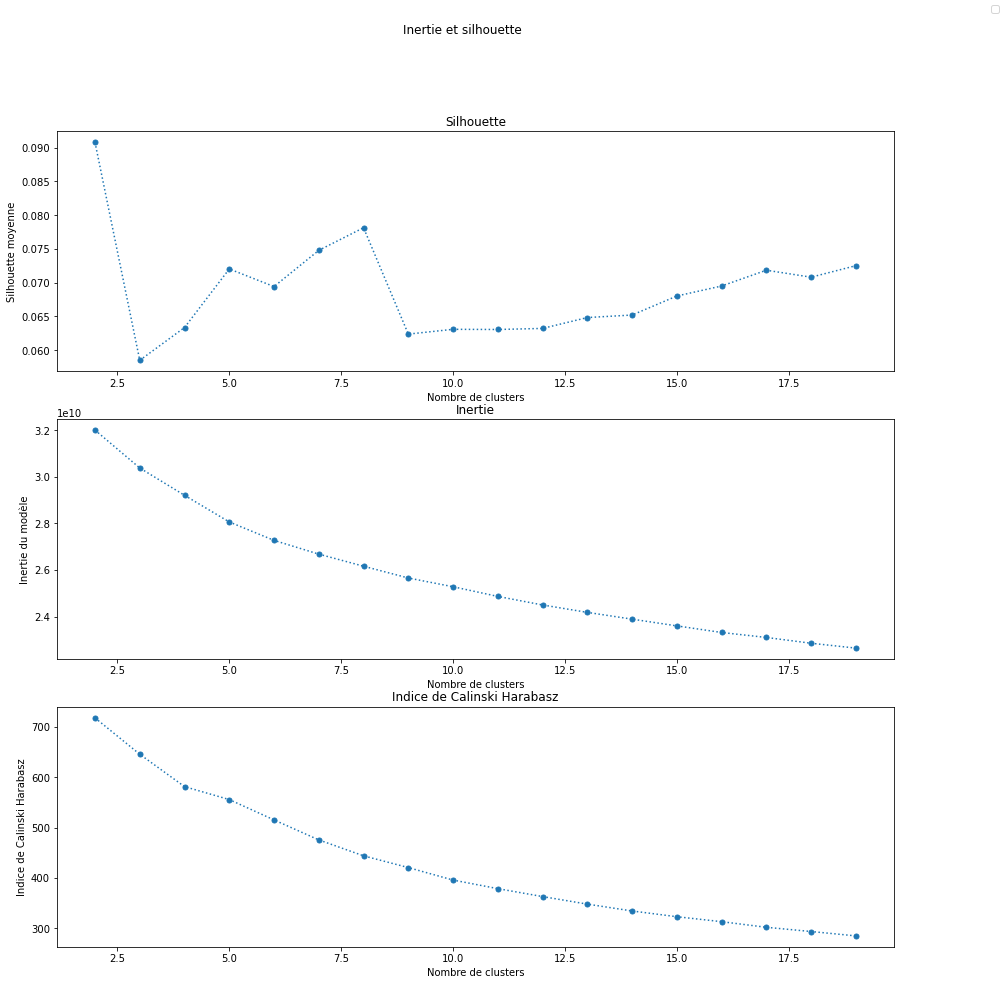
\includegraphics[width=0.85\textwidth]{"./Images/CH.png"}
	\caption{\centering Indice de Calinski-Harabasz avec l'inertie et la silhouette moyenne du modèle en fonction du nombre de clusters (K)}
	\label{fig:CH}
\end{figure}


\paragraph{Davies Bouldin} L'indice de Davies-Bouldin quand à lui évalue la qualité de la partition en fonction de la distance entre les centroïdes des clusters et la distance intra-cluster. L'indice de Davies-Bouldin est calculé pour chaque partition et pour chaque k. La partition qui a la valeur minimale de l'indice de Davies-Bouldin est considérée comme la partition optimale.

\begin{figure}[H]
	\centering
	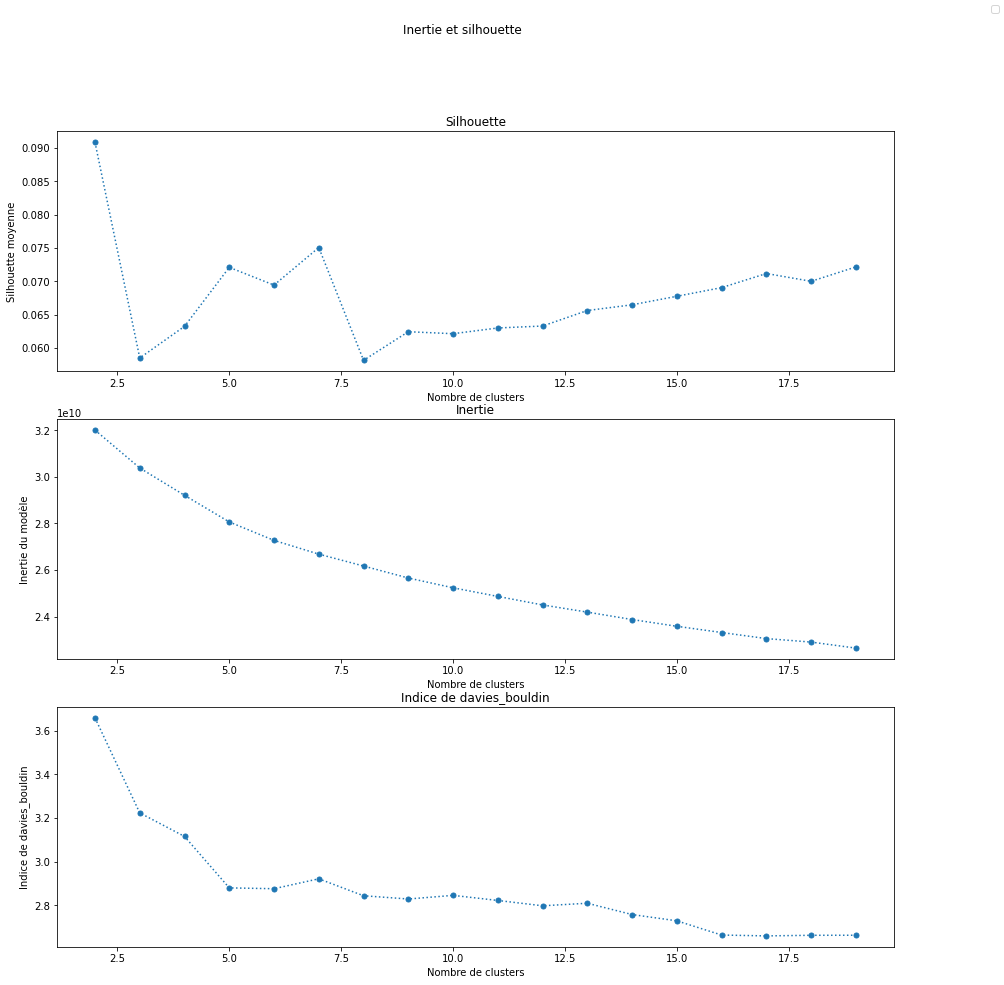
\includegraphics[width=0.85\textwidth]{"./Images/DB.png"}
	\caption{\centering Indice de Davies Bouldin avec l'inertie et la silhouette moyenne du modèle en fonction du nombre de clusters (K)}
	\label{fig:DB}
\end{figure}

En résumé, nous avons exploité plusieurs indicateurs qui permettent, en théorie, de déterminer le nombre de clusters optimal pour notre problème. En pratique, nous avons vu que les indicateurs de Calinski-Harabasz et de Davies Bouldin pris individuellement ne donnent pas de solution à ce problème, car dans un cas le K théorique optimal est 2, ce qui nous semble trop peu pour être raisonnablement un nombre de clusters optimal, et dans l'autre cas le K théorique optimal est 20, qui nous semble être trop grand.

En revanche, la mise en parallèle des graphiques obtenus pour ces deux indices, ainsi que celui obtenu pour la silhouette, permet de mettre en lumière une solution optimale en cherchant un compromis entre un K trop grand qui donne un faible indice de Calinski-Harabasz et un K trop petit qui donne un indice de Davies Bouldin trop élevé. Ce nombre semble être 7.


\subsection{Avec des labels !}
L'information la plus regardée dans le cas d'une étude sérieuse serait très probablement le pourcentage moyen d'erreurs. Or il n'est possible de l'obtenir qu'à condition de travailler sur une base de données étiquettées.  \\

\alertinfo{Dans le cas où nous définissons plus de 10 clusters nous utilisons une fonction de pré-traitement qui associe une étiquette (entre 0 et 9) à chaque cluster. Pour décider nous choisissons d'associer l'étiquette de la classe la plus représentée (par rapport aux vraies étiquettes) dans chacun de ces clusters. Nous calculons ensuite l'erreur à partir de ces 10 représentations.}

\begin{figure}[H]
	\centering
	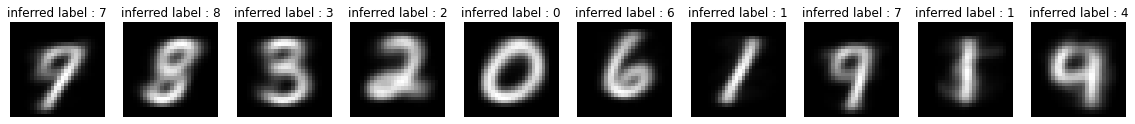
\includegraphics[width=0.85\textwidth]{"./Images/inf.png"}
	\caption{\centering Le centre des cluster avec les clases inférés}
\end{figure}


\alerterror{On remarque ici que les labels inférés sont proche de ce que l'on peut observer mais pas parfaitement bon, c'est ici la limite des Kmeans...}

On peut donc maintenant aussi calculer le pourcentage d'erreur de mauvaise classification, puisque l'on a les labels des classes. On obtient les graphs si dessous : 

\begin{figure}[H]
	\centering
	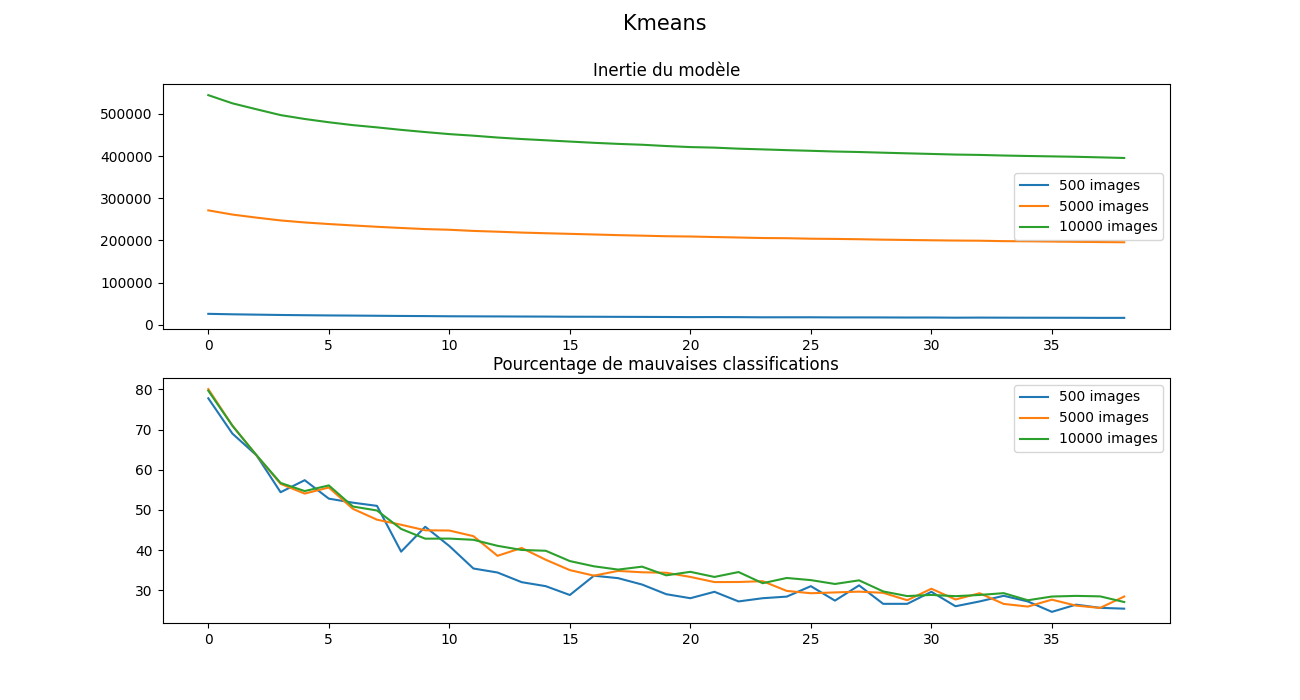
\includegraphics[width=0.85\textwidth]{"./Images/Kmeans_no_prepo_erreur.png"}
	\caption{\centering Le centre des cluster avec les clases inférés}
\end{figure}

Le pourcentage d'erreur diminueavec le nombre de clusters. Un même chiffre pouvant s'écrire de plusieurs façons, (sept avec et sans barre par exemple) l'association initiale en 10 clusters présentée précédemment permet de les classer à la fin comme un même chiffre. Que cette erreur diminue avec le nombre de clusters est donc également cohérent.\\
Les pourcentage d'erreurs de classifications augmentent cependant avec la taille de la base de données, il serait intéressant de chercher à savoir si cette tendance se confirme avec davantage de clusters (jusqu'à 250) et d'images.

\subsection{Kmedoids}

Nous allons maintenant passer à l'algorithme Kmedoids. La première comparaison vient à être fait sur la qualité des centres des clusters. On obtient alors avec 10 clusters (comme nous l'avions fait avec le Kmeans) le résultat suivant :
\begin{figure}[H]
	\centering
	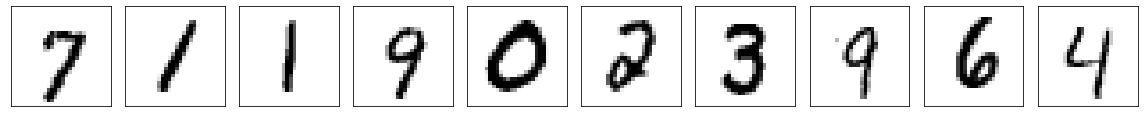
\includegraphics[width=0.85\textwidth]{"./Images/kmc.png"}
	\caption{\centering Centre des clusters du Kmedoids avec 10 clusters}
\end{figure}

On peut remarquer ici :
\begin{itemize}
	\item Sur les 10 centre de clusters on retrouve 8 chiffres, là ou avec le Kmeans on trouve 7 classes. On peut donc estimer que l'algorithme du Kmedoids est plus performant ici.
	\item Du point de vu temps, l'algorithme du Kmeans met 4s là ou le Kmedoids à mis 3.4s on peut donc aussi le considérer plus performant d'un point de vu temporel sur un échantillon de 10 000 images.
\end{itemize}

Suite à ces résultats il nous semble important que considérer les performances de nos deux algorithmes en prenant en compte le nombre de données utilisé pour l'entrainement. On considèrera donc 3 test avec 500 images, 5000 images et 10 000 images. \\

On refait donc les tests vu précédemment pour le Kmeans avec notre nouvel algorithme :

\begin{figure}[H]
	\centering
	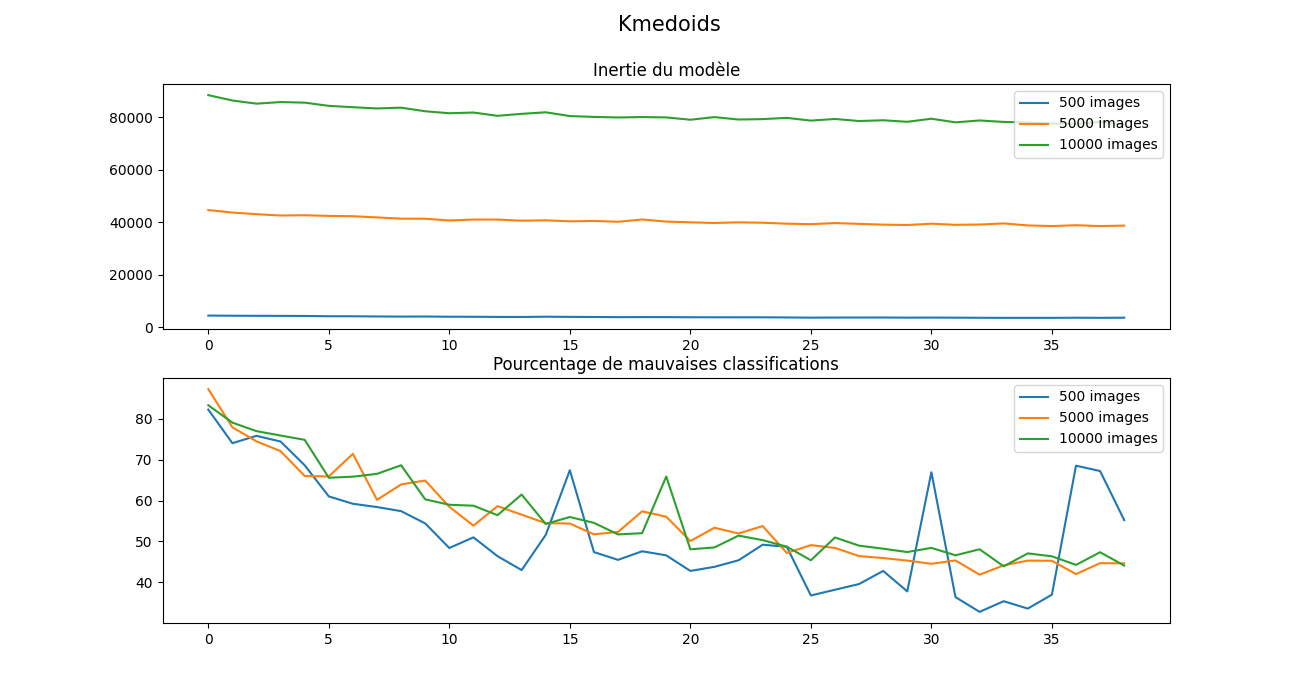
\includegraphics[width=0.85\textwidth]{"./Images/Kmedoids_no_prepo_erreur.png"}
	\caption{\centering Kmedoids et erreur de classification}
\end{figure}
\begin{figure}[H]
	\centering
	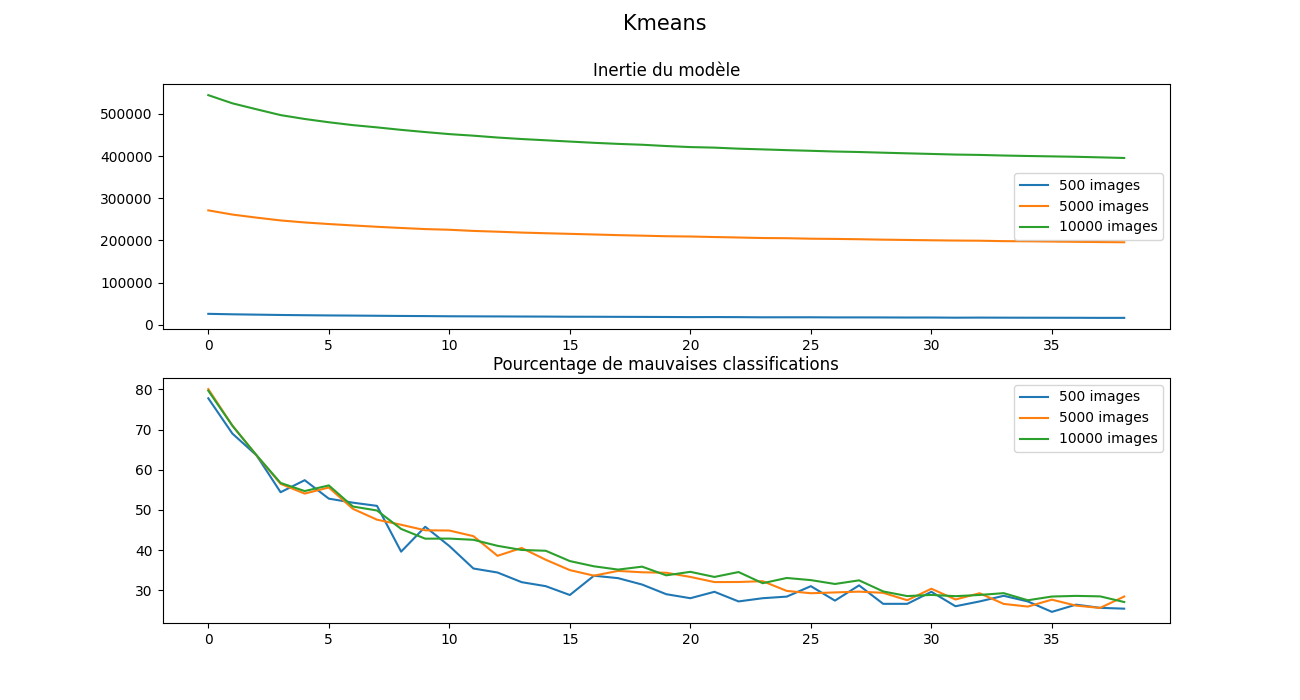
\includegraphics[width=0.85\textwidth]{"./Images/Kmeans_no_prepo_erreur.png"}
	\caption{\centering Le centre des cluster avec les clases inférés}
\end{figure}

Face à ces résultats l'algorithme du Kmeans semble plus performant sur ce jeu de données. En effet, le pourcentage de mauvaise classification semble bien converger et diminuer avec le nombre de cluster. Même si nous avons vu que cette métrique seule ne suffit pas, il semble que Kmedoids ne performe pas aussi bien. Tout comme il est intéressant de noter qu'avec 10 000 images l'algorithme du Kmedoids semble ne pas vraiment converger en terme d'erreur de classification...
\\
Par ailleurs, durant toutes ces itérations il a été notable que Kmeans est plus lent que Kmedoids, surtout sur de petites base de données. Leur temps de calcul respectif se rapprochent cependant avec l'augmentation du nombre de matrices considérées, et pour 10000 images Kmeans commence à passer devant Kmedoids. (Au delà Kmeans est d'ailleurs beaucoup plus rapide). \\
 Pour chaque image l'algorithme Kmedoids converge bien plus rapidement que Kmeans. (En moyenne sa convergence 10 fois plus rapide). Cette tendance diminue en revanche avec la taille du dataset.
 \alertinfo{Au delà de 20000 images Kmedoids devenait beaucoup trop lent. Et augmenter encore le nombre d'images ne présente pas tant d'intérêt en terme de performances (du fait de la ressemblance des images, c'est pourquoi nous avons choisi ces tailles de base de données).}

\section{Annexe}

\subsection{Codes}
L'ensemble des fonctions, modules et figures utilisés pour réaliser ou approfondir ce TP sont disponibles à l'adresse suivante : \href{https://github.com/CharlesFarhat/coursTSP/tree/2A/MAT4102/TP_Kmeans}{\underline{\textit{https://github.com/CharlesFarhat/coursTSP/tree/2A/MAT4102/TP\_Kmeans}}}

\subsection{Références}

[1] : \url{http://www.xavierdupre.fr/app/mlstatpy/helpsphinx//c_clus/kmeans.html#id31}

[2] : \url{https://scikit-learn.org/stable/modules/generated/sklearn.metrics.silhouette_score.html}

\end{document}